\documentclass[11pt,a4paper]{article}
\usepackage[T1]{fontenc}
\usepackage[utf8]{inputenc}

\usepackage[protrusion=false,expansion=false]{microtype}
\usepackage{amsmath,amssymb,amsthm,mathtools}
\usepackage{stmaryrd}
\usepackage{mathpartir}
\usepackage{tikz}
\usetikzlibrary{arrows.meta,positioning,calc,decorations.pathmorphing}
\usepackage{listings}
\usepackage{xcolor}
\usepackage{booktabs}
\usepackage{enumitem}
\usepackage[margin=2.6cm]{geometry}
\usepackage[hidelinks]{hyperref}

% ---------------------------------------------------------------------------
% Macros
% ---------------------------------------------------------------------------
\newcommand{\N}{\mathbb{N}}
\newcommand{\Z}{\mathbb{Z}}
\newcommand{\Fin}{\mathit{Fin}}
\newcommand{\List}{\mathit{List}}
\newcommand{\Set}{\mathbf{Set}}
\newcommand{\Cont}{\mathbf{Cont}}
\newcommand{\Poly}{\mathbf{Poly}}
\newcommand{\cont}[2]{(#1 \triangleleft #2)}
\newcommand{\ext}[1]{T_{#1}}
\newcommand{\jmeq}{\mathrel{\stackrel{\mathit{jm}}{=}}}
\newcommand{\eqmor}{\mathrel{\stackrel{\mathit{eqmor}}{=}}}
\newcommand{\monus}{\mathbin{\dot{-}}}
\newcommand{\todo}[1]{{\color{red}\textbf{[TODO: #1]}}}
\newcommand{\coq}[1]{\texttt{#1}}
\newcommand{\fn}[1]{\ensuremath{\mathit{#1}}}
\newcommand{\rev}{\ensuremath{\mathit{rev}}}
\newcommand{\app}{\ensuremath{\mathbin{+\!\!+}}}
\newcommand{\lens}{\Rightarrow}
\newcommand{\mmap}{\fn{mmap}}
\newcommand{\reduce}{\fn{reduce}}
\newcommand{\lastk}{\ensuremath{\mathit{last}_k}}

\lstdefinelanguage{Coq}{
  morekeywords={Inductive,Fixpoint,Definition,Lemma,Theorem,Proof,Qed,match,with,end,fun,forall,return,in,if,then,else,let,Ltac,Set,Prop,Type,Record,nat,Corollary},
  sensitive=true,
  morecomment=[s]{(*}{*)},
  morestring=[b]",
}
\lstset{language=Coq,basicstyle=\small\ttfamily,keywordstyle=\bfseries,
  commentstyle=\itshape\color{black!60},columns=fullflexible,keepspaces=true,
  frame=none,xleftmargin=1em,breaklines=true,showstringspaces=false}

\theoremstyle{plain}
\newtheorem{theorem}{Theorem}[section]
\newtheorem{proposition}[theorem]{Proposition}
\newtheorem{lemma}[theorem]{Lemma}
\newtheorem{corollary}[theorem]{Corollary}
\theoremstyle{definition}
\newtheorem{definition}[theorem]{Definition}
\newtheorem{example}[theorem]{Example}
\newtheorem{observation}[theorem]{Observation}
\theoremstyle{remark}
\newtheorem{remark}[theorem]{Remark}

\title{Arithmetic Analysis of Polymorphic Programs\\
  \large and the Verification of Typed Agent Interfaces}
\author{Rawle Prince\thanks{Tucan Analytics Ltd, London, United Kingdom.
    \texttt{rawle.prince@tucan-analytics.com}. The original version of this work was carried out
    while the author held a departmentally funded research studentship in the School of
    Computer Science, University of Nottingham, between 10/2006 and 09/2010.}}
\date{Revised version, October 2026}

\begin{document}
\maketitle

\begin{abstract}
We exploit the representation of data types as container functors to develop a
decision procedure for a large class of polymorphic functions on lists.  A container
describes a data type by the \emph{shapes} its values can take and, for each shape, the
\emph{positions} at which data are stored; a representation theorem guarantees that every
polymorphic function between container types is given by a map on shapes together with a
family of maps on positions.  For lists, shapes are natural numbers and positions are
finite types.  We show that the behaviour of the dependently typed position maps can be
captured by functions on the natural numbers, and that when both shape and position maps
are definable in Presburger arithmetic, equality of polymorphic functions reduces to the
validity of universally quantified formulae of Presburger arithmetic, which is decidable.
The procedure is implemented as a Coq tactic that discharges the standard identities
between list functions (reversal, appending, taking, dropping, rotation, \ldots) without
induction, each in a fraction of a second.

We also develop a second reading of the same mathematics.  
A container is also the type of an \emph{interface}: the moves an agent can emit and, for each move,
the responses it accepts.  Container morphisms are then \emph{adapters} between
interfaces (dependent lenses), and the composition of adapters is the composition of
container morphisms.  Interfaces whose shape is a count --- batches of tool calls,
context windows, ranked candidate lists --- are list-shaped, and the adapters between
them are exactly the list morphisms that our procedure decides.  We show that arithmetic
equality of adapters implies behavioural equality of every agent wrapped by them, that
losslessness (cartesianness) of an adapter is decidable, and we verify, and in two
cases refute, invariants of sliding context windows and of fan-out/fan-in routing.  The
accompanying Coq development is new, self-contained and axiom-free.
\end{abstract}

% ===========================================================================
\section{Introduction}\label{sec:intro}
% ===========================================================================

Techniques for reasoning about polymorphic functions have applications that range from
specification and verification, through model checking and testing, to the certification
of mobile code.  This paper presents a way of reasoning about polymorphic functions that
is based on the representation of data types as \emph{containers}
\cite{Abbott03,AbbottAltenkirchGhani03,AbbottAltenkirchGhani05}.  A container describes a
concrete data type by two pieces of information: the \emph{shapes} that values of the
type can take, and, for each shape, the set of \emph{positions} at which data are stored.
A list, for instance, has as shape its length $n$ and as positions the $n$ slots
$0,\dots,n-1$; a binary tree has as shape a tree with no data in it, and as positions the
nodes of that tree.  A value of the type is then a shape together with an assignment of a
datum to each position.

Earlier presentations of container theory used the language of category theory
\cite{AbbottAltenkirchGhani03,AbbottAltenkirchGhani05} and investigated its applications
to generic programming \cite{AltenkirchMcBrideMorris07,Morris07}.  Our interest comes from
automated reasoning, and is motivated by the ability of containers to simplify reasoning
tasks \cite{AbbottAltenkirchGhaniMcBride04,PrinceGhaniMcBride08}.  The basis of everything
that follows is the \emph{representation theorem} for containers: every polymorphic
function (natural transformation) between container types is given by a map on shapes
and, contravariantly, a family of maps on positions.  For instance, a polymorphic function
$F : \List\,X \to \List\,X$ is represented by a pair
\[
  \big(\;u : \N \to \N,\quad f : \textstyle\prod_{n:\N}\, \Fin\,(u\,n) \to \Fin\,n\;\big),
\]
where $u$ computes the length of the output from the length of the input, and, for each
input length $n$, the \emph{reindexing map} $f_n$ says from which position of the input
each position of the output is fetched.  Here $\Fin\,n$ is the type with exactly $n$
elements, which we think of as $\{0,\dots,n-1\}$.  Reversal, for example, keeps the length
($u\,n = n$) and fetches output position $i$ from input position $n - i - 1$.

Many functions on lists are, in this representation, nothing but arithmetic on lengths and
indices.  This was the insight behind Bundy and Richardson's \emph{ellipsis}
technique \cite{BundyRichardson99}, in which lists are written as
$x_1,\dots,x_n$ and functions are specified by what they do to indices, and it was
developed further, with containers as the formal underpinning, in
\cite{PrinceGhaniMcBride08}.  Those developments were carried out in a dependently typed
setting, where indices live in the finite types $\Fin\,n$.  Dependent types are what make
the representation \emph{correct by construction} --- an index into a list of length $n$
cannot exceed $n-1$ --- but they are also what prevents the direct use of decision
procedures, which operate on natural numbers or integers, not on families of finite types.

\subsection{Contribution: arithmetic verification}

The first contribution of this paper is to show that, for lists, nothing is lost by
abandoning dependent types at the point where decision procedures are needed.  The
behaviour of a reindexing map $f : \prod_n \Fin(u\,n) \to \Fin\,n$ is captured by a
function $g : \N \times \N \to \N$ on natural numbers together with a side condition
(the index is in range), and equality of two polymorphic functions becomes a statement of
the form
\[
  \forall n.\; u\,n = v\,n \;\wedge\; \forall n\,i.\; i < u\,n \to g_1\,n\,i = g_2\,n\,i .
\]
When $u$, $v$, $g_1$ and $g_2$ are definable in Presburger arithmetic --- the first-order
theory of the natural numbers with addition, which is decidable \cite{Presburger29} --- so
is this statement, and because it has a universal prefix and a quantifier-free matrix it
falls into the fragment handled efficiently by the Omega test \cite{Pugh91}, by Coq's
\coq{lia} tactic and by SMT solvers.  We identify a class of
\emph{Presburger-definable morphisms}, closed under composition, that covers the
familiar functions on lists (\S\ref{sec:arith}), and we implement a Coq tactic that proves
the identities of Figure~\ref{fig:properties} automatically.

\subsection{Contribution: typed agent interfaces}

The second contribution was prompted by an observation of Ghani \cite{GhaniPodcast26}.  
An \emph{AI agent} responds to prompts: it has a type of
possible outputs (moves, tool calls, messages) and, for each output, a type of inputs it
is prepared to receive next.  That is a container.  The whole theory of containers ---
and its continuation as the theory of polynomial functors by Spivak and
Niu \cite{Spivak20,NiuSpivak24} --- therefore applies to the \emph{interfaces} of agents.
In particular, a container morphism $\cont{S}{P} \lens \cont{S'}{P'}$ is a protocol
\emph{adapter}: it translates the moves of one interface into those of another
(covariantly) and routes responses back (contravariantly).  In the terminology of
\cite{NiuSpivak24} it is a \emph{dependent lens}.  Composition of adapters is composition
of container morphisms, and wrapping an agent by an adapter is the extension of the
container morphism applied to the agent's one-step behaviour.

Most of today's agentic systems are untyped: an LLM has, as Ghani puts it, type
``string to string'', and orchestration frameworks pass around lists of messages and
JSON objects whose shapes are checked, if at all, at run time.  A \emph{typed} agentic
system, of the kind being built at Kodamai \cite{KodamaiEEJ26,GhaniPodcast26}, assigns
container types to interfaces and composes agents along typed adapters.  Once that is
done, a familiar dividend of types becomes available: to check that two ways of wiring a
system agree, or that an adapter preserves information, one checks the types and the
adapters, not the agents.

Here is where the first contribution meets the second.  A great many agent interfaces are
\emph{list-shaped}: an orchestrator that fans out $n$ tool calls and fans in $n$
results; a conversation whose context is a window over a history of length $n$; a
retriever that returns $k$ ranked documents.  Adapters between list-shaped interfaces
are list morphisms --- truncate, drop the oldest, reverse the ranking, split and merge a
batch --- and they are exactly the Presburger-definable morphisms of
\S\ref{sec:arith}.  Consequently, (i) equality of two adapter pipelines is decidable;
(ii) losslessness of an adapter (no response dropped or duplicated) is decidable; and
(iii) by functoriality, an equation between adapters transfers to every agent wrapped by
them.  We prove these facts in Coq (\S\ref{sec:agents-verif}) and verify, in well under a second,
invariants of sliding context windows and of fan-out/fan-in routing; just as usefully,
the procedure \emph{refutes} two plausible-looking adapter laws, exhibiting the
counterexamples.

\subsection{What is new since the original vesion}

The arithmetic core (\S\ref{sec:containers}--\S\ref{sec:arith}) is a thoroughly revised
version of the original work \cite{Prince10}.\footnote{Note, the orignal work can be found here: \url{https://github.com/rawlep/ArithmeticAnaysisOfPolymorphicPrograms} and also appears in the \texttt{legacy} folder in the updated repository (\S\ref{sec:notation}).} 
Beyond presentational changes, the mathematics has been tightened in three places: the
decidability theorem now comes with a proof (Theorem~\ref{thm:decidable}); correctness of
composition is stated and proved (Theorem~\ref{thm:comp}); and two definitions of the
orignal Coq development that were found to be wrong (\fn{take} and the position map of
$\app$) are corrected, with every property re-proved for the corrected definitions
(\S\ref{sec:coq}).  The Coq development is a complete rewrite: it is self-contained,
axiom-free, uses \coq{lia} in place of the deprecated \coq{omega}, and proves each
identity of Figure~\ref{fig:properties} in at most a few hundred milliseconds, where the
original code took between 6 and 75 seconds.  It also demomstrates how the container-style 
definitions are connected with ordinary recursive definitions: \emph{transfer lemmas} 
relate each morphism to the corresponding function of the Coq
standard library, and standard theorems about ordinary lists are derived from the decision
procedure without induction.  Sections~\ref{sec:agents} and~\ref{sec:agents-verif}, and
most of \S\ref{sec:related}, are new.

\subsection{Notation and conventions}\label{sec:notation}

We use two notations side by side, and we say which is which.  Mathematical statements and
definitions are written in a type-theoretic notation in the style of Agda and
Epigram \cite{McBrideMcKinna04}: $\sum_{s:S} P\,s$ (or $\sum s : S.\, P\,s$) is the type of
dependent pairs $(s, p)$ with $s : S$ and $p : P\,s$; $\prod_{s:S} P\,s$ is the type of
dependent functions $f$ with $f\,s : P\,s$ for every $s$; and a definition by pattern
matching lists one clause per constructor, with the \emph{absurd clause} ``$!$''
marking a case that cannot arise (written \verb|()| in Agda).  Code from the accompanying
development is shown in Coq syntax in typewriter font.  In Coq, $\sum$ is \coq{sigT} or
\coq{\{x : A \& B x\}} and $\prod$ is \coq{forall}.  We write $S\,n$ for the successor of
$n$ in pattern-matching clauses and $n + 1$ in arithmetic; the two are identical.
Cut-off subtraction on $\N$, written $n \monus m$ and equal to $0$ when $m \ge n$, is
the subtraction of Coq's \coq{nat}.  Lists are indexed from $0$ throughout.

\paragraph{Accompanying development.}  All definitions and results marked
\textsf{[Coq]} are formalised in the development (directory \texttt{theories/}) at
\begin{center} % need to update this 
  \url{https://github.com/tucananalytics/ArithmeticAnalysisOfPolymorphicProgramsAndTypedAgentInterfaces}
\end{center}
of which \S\ref{sec:coq} gives an overview.

% ===========================================================================
\section{Containers}\label{sec:containers}
% ===========================================================================

We begin with an informal motivation, then give the definitions we need.  Readers familiar
with containers may skip to \S\ref{sec:rep-eq}; readers wishing to see the full theory
should consult \cite{AbbottAltenkirchGhani05}.

\subsection{Motivation: unique representations of lists}\label{sec:motivation}

Bundy and Richardson \cite{BundyRichardson99} represent a list of elements of type
$\tau$ by a length and a function that produces its elements:
\begin{align*}
  \Box &: \N \to (\N \to \tau) \to \List\,\tau \\
  \Box\,(0, f) &= [\,] \\
  \Box\,(S\,n, f) &= f\,1 :: \Box\,(n, f \circ S).
\end{align*}
Thus $\Box(n, f)$ is the list $[f\,1, f\,2, \dots, f\,n]$, and functions on lists can
often be written as arithmetic on $n$ and on the arguments of $f$.  The difficulty with
this representation is that $\Box$ is not injective: the lists $\Box(2, f)$ and
$\Box(2, f')$ are equal as soon as $f$ and $f'$ agree on $1$ and $2$, regardless of whatever they do
elsewhere, so a list has many representations and $f$ carries information that is never
observed.  The cure is to restrict the domain of $f$ to the positions that exist, that is,
to make its domain depend on $n$.  By the use of the finite type
\begin{lstlisting}
Inductive Fin : nat -> Set :=
  | fz : forall n, Fin (S n)
  | fs : forall n, Fin n -> Fin (S n).
\end{lstlisting}
(so $\Fin\,0$ is empty, and $\Fin(S\,n)$ has the elements $\fn{fz}$ and $\fn{fs}\,i$ for
$i : \Fin\,n$ --- we write $\fn{fs}$ in italics to avoid reading it as an application
$f\,s$), the type
\[
  \Phi\,X \;=\; \textstyle\sum_{n:\N}\, (\Fin\,n \to X)
\]
represents lists uniquely: a pair $(n, f)$ with $f : \Fin\,n \to X$ determines the list
$[f\,0, \dots, f\,(n-1)]$ and is determined by it.  $\Phi$ is a functor, with
$\Phi\,g\,(n, f) = (n, g \circ f)$.  It turns out that $\Phi$ is precisely the
representation of lists that container theory produces.

\subsection{Containers and their extensions}

\begin{definition}[Container]\label{def:container}
  A \emph{container} $\cont{S}{P}$ consists of a type $S$ of \emph{shapes} and, for each
  shape $s : S$, a type $P\,s$ of \emph{positions}.
\end{definition}

We sometimes write a container in pointwise form, $(s : S \triangleleft P\,s)$, to make
the shape variable explicit.  The \emph{list container} is
$(n : \N \triangleleft \Fin\,n)$: a shape is a length and the positions of a list of
length $n$ are its $n$ slots.  The container of binary trees has as shapes the trees with
no data %(the type $\fn{Btree}\,\mathbf{1}$) 
and as positions, for each such tree, its nodes.

\begin{definition}[Extension]\label{def:extension}
  The \emph{extension} of a container $\cont{S}{P}$ is the functor
  $\ext{\cont{S}{P}} : \Set \to \Set$ defined by
  \[
    \ext{\cont{S}{P}}\,X \;=\; \textstyle\sum_{s:S}\, (P\,s \to X),
  \]
  with action on functions $\ext{\cont{S}{P}}\,g\,(s,h) = (s, g \circ h)$.
\end{definition}

A value of $\ext{\cont{S}{P}}\,X$ is a shape together with an assignment of an element of
$X$ to every position of that shape.  For the list container,
$\ext{(\N \triangleleft \Fin)}\,X = \sum_n (\Fin\,n \to X) = \Phi\,X \cong \List\,X$.

\begin{remark}[Calculating shapes]\label{rem:shapes}
  The shapes of an algebraic data type can be read off by setting the payload type to the
  unit type: the shape type of $\List\,X$ is $\List\,\mathbf{1} \cong \N$ and that of
  $\fn{Btree}\,X$ is $\fn{Btree}\,\mathbf{1}$.  Containers are closed under the
  constructions of strictly positive types, given by the grammar
  \[
    \tau \;::=\; X \;\mid\; \mathbf{0} \;\mid\; \mathbf{1} \;\mid\; \tau + \tau \;\mid\;
    \tau \times \tau \;\mid\; K \to \tau \;\mid\; \mu X.\,\tau ,
  \]
  in which $X$ ranges over type variables, $\mathbf{0}$ and $\mathbf{1}$ are the empty and
  unit types, $+$ and $\times$ are sum and product, $K \to \tau$ is exponentiation by a
  constant type $K$ (one with no free variables), and $\mu X.\,\tau$ forms the least
  fixed point, that is, the inductive type whose constructors are described by $\tau$
  with $X$ standing for recursive occurrences.  For example,
  $\N = \mu X.\, \mathbf{1} + X$, $\List\,A = \mu X.\, \mathbf{1} + A \times X$ and
  $\fn{Btree}\,A = \mu X.\, A + X \times X$.  See \cite{AbbottAltenkirchGhani05} for the
  construction of the container corresponding to each clause.
\end{remark}

\subsection{Container morphisms}\label{sec:morphisms}

A polymorphic function between container types, say $\rev : \List\,X \to \List\,X$, is
determined by what it does to shapes and positions: $\rev$ keeps the length, and the datum
at output position $i$ is the datum at input position $n - i - 1$.  Note the direction of
the second map: it goes from \emph{output} positions to \emph{input} positions.  This is
deliberate.  A polymorphic function cannot invent data, so every output position must be
filled from some input position --- hence a function from output positions to input
positions.  The opposite direction would not work in general: $\fn{tail}$ discards input
position $0$, which has nowhere to go (Figure~\ref{fig:tail}), and a function that
duplicates its input sends one input position to two output positions, which is not a
function at all.

\begin{figure}[t]
  \centering
  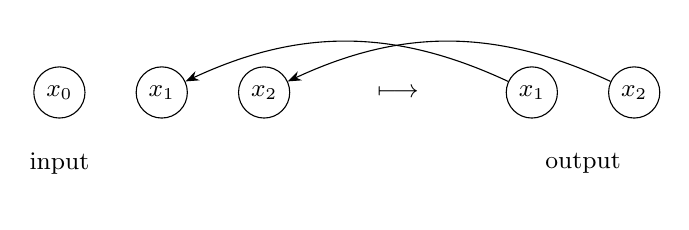
\begin{tikzpicture}[every node/.style={circle,draw,minimum size=6.5mm,inner sep=0pt,font=\small}]
    \node (a0) at (0,0) {$x_0$};
    \node (a1) at (1.3,0) {$x_1$};
    \node (a2) at (2.6,0) {$x_2$};
    \node (b1) at (6,0) {$x_1$};
    \node (b2) at (7.3,0) {$x_2$};
    \node[draw=none] at (4.3,0) {$\longmapsto$};
    \draw[-{Stealth},bend right=25] (b1) to (a1);
    \draw[-{Stealth},bend right=25] (b2) to (a2);
    \node[draw=none,font=\small] at (0,-0.9) {input};
    \node[draw=none,font=\small] at (6.65,-0.9) {output};
  \end{tikzpicture}
  \caption{The reindexing map of $\fn{tail}$ sends each output position back to the input
    position it is fetched from.  Input position $0$ has no preimage: its datum is
    discarded.}\label{fig:tail}
\end{figure}

\begin{definition}[Container morphism]\label{def:cmor}
  A \emph{container morphism} $(u, f) : \cont{S}{P} \lens \cont{S'}{P'}$ consists of
  \[
    u : S \to S' \qquad\text{and}\qquad f : \textstyle\prod_{s:S}\, P'\,(u\,s) \to P\,s .
  \]
  We call $u$ the \emph{shape map} and $f$ the \emph{position} or \emph{reindexing map}.
\end{definition}

The shape map is covariant (it follows the direction of the function) and the position map
is contravariant, for the reason just given.  Each container morphism determines a
polymorphic function, its extension:
\begin{equation}\label{eq:mmap}
  \mmap\,(u,f) : \ext{\cont{S}{P}}\,X \to \ext{\cont{S'}{P'}}\,X, \qquad
  \mmap\,(u,f)\,(s, g) = (u\,s,\; g \circ f_s).
\end{equation}
In words: apply $u$ to the shape, and fill output position $p$ with the datum
$g\,(f_s\,p)$ found at the input position $f_s\,p$.

\begin{example}[Reverse]\label{ex:rev}
  $\fn{crev} = (\fn{id}, \fn{rv}) : (\N \triangleleft \Fin) \lens (\N \triangleleft \Fin)$,
  where $\fn{rv}_n\,i$ is the element of $\Fin\,n$ with value $n - i - 1$.  In the
  dependently typed style $\fn{rv}$ is defined by recursion on the index, using the
  functions $\fn{top}_n : \Fin(S\,n)$ (the largest element, of value $n$) and
  $\fn{emb}_n : \Fin\,n \to \Fin(S\,n)$ (the value-preserving embedding):
  \begin{align*}
    \fn{rv}_{S\,n}\,\fn{fz} &= \fn{top}_n &
    \fn{top}_0 &= \fn{fz} & \fn{emb}\,\fn{fz} &= \fn{fz}\\
    \fn{rv}_{S\,n}\,(\fn{fs}\,i) &= \fn{emb}\,(\fn{rv}_n\,i) &
    \fn{top}_{S\,n} &= \fn{fs}\,\fn{top}_n & \fn{emb}\,(\fn{fs}\,i) &= \fn{fs}\,(\fn{emb}\,i).
  \end{align*}
  Every element of $\Fin(S\,n)$ is either $\fn{top}_n$ or $\fn{emb}\,i$ for a unique $i$;
  this is the \emph{view} \cite{McBride00,McBrideMcKinna04} used in the Coq code of
  \S\ref{sec:coq}.
\end{example}

\begin{example}[Tail]\label{ex:tail}
  $\fn{ctail} = (u, f)$ with $u\,0 = 0$, $u\,(S\,n) = n$, $f_0 = \;!$ (no output
  positions when the input is empty) and $f_{S\,n}\,i = \fn{fs}\,i$ (output position $i$
  is fetched from input position $i + 1$).
\end{example}

\begin{definition}[Cartesian morphism]\label{def:cartesian}
  A container morphism $(u,f)$ is \emph{cartesian} if every $f_s : P'(u\,s) \to P\,s$ is a
  bijection.
\end{definition}

A cartesian morphism rearranges data without loss or duplication; $\fn{crev}$ is
cartesian, $\fn{ctail}$ is not.  Note that cartesianness constrains the \emph{position}
maps only; the shape map $u$ may well fail to be injective (\S\ref{sec:conclusion}
returns to this point).

\begin{definition}[Composition]\label{def:comp}
  Given $(u_1, f_1) : \cont{S}{P} \lens \cont{S'}{P'}$ and
  $(u_2, f_2) : \cont{S'}{P'} \lens \cont{S''}{P''}$, their composite
  $(u_2, f_2) \circ (u_1, f_1) : \cont{S}{P} \lens \cont{S''}{P''}$ is
  $(u_2 \circ u_1,\; \lambda s\,p.\; f_1\,s\,(f_2\,(u_1\,s)\,p))$.
\end{definition}

Shapes are mapped forwards through $u_1$ then $u_2$; a position of the final output is
routed backwards through $f_2$ then $f_1$.  Containers and container morphisms form a
category $\Cont$ \cite{AbbottAltenkirchGhani05}, and $\mmap$ respects composition and
identities (\textsf{[Coq]} \coq{mmap\_comp}, \coq{mmap\_id}).

\subsection{The representation theorem and equality}\label{sec:rep-eq}

\begin{theorem}[Representation \cite{AbbottAltenkirchGhani03,AbbottAltenkirchGhani05}]\label{thm:rep}
  The map $\mmap$ is a bijection between container morphisms
  $\cont{S}{P} \lens \cont{S'}{P'}$ and natural transformations
  $\ext{\cont{S}{P}} \to \ext{\cont{S'}{P'}}$.
\end{theorem}

Categorically the theorem is an instance of the Yoneda lemma, and it says that
$T : \Cont \to [\Set, \Set]$ is a full and faithful embedding.  For us it says two things.
First, \emph{every} polymorphic function between lists is of the form
$\mmap\,(u, f)$, so nothing is lost by working with shape and position maps.  Second,
two container morphisms with the same extension are equal, so an equation between
polymorphic functions can be proved by proving an equation between container morphisms.
(The core theory, including this theorem, was formalised in Coq in \cite[Ch.~4]{Prince10}.)

Stating the equality requires some care.  Two container morphisms
$(u, f), (u', f') : \cont{S}{P} \lens \cont{S'}{P'}$ have components of types
\[
  u, u' : S \to S', \qquad
  f : \textstyle\prod_s P'(u\,s) \to P\,s, \qquad
  f' : \textstyle\prod_s P'(u'\,s) \to P\,s .
\]
Two issues arise.  \emph{Heterogeneity}: $f$ and $f'$ have different types unless one
already knows $u = u'$, so the ordinary (homogeneous) equality of type theory cannot even
be used to state $f = f'$.  \emph{Extensionality}: we wish to regard two functions as
equal when they agree on all arguments, not only when they have the same definition.

The standard remedy for the first issue is McBride's heterogeneous equality
\cite{McBride99,McBride00}, written $a \jmeq b$ and also called ``John Major equality''.
Its rules are:
\begin{mathpar}
  \inferrule{a : A \\ b : B}{a \jmeq b : \fn{Prop}}
  \and
  \inferrule{a : A}{\fn{refl} : a \jmeq a}
  \and
  \inferrule{a : A \\ \Phi : \forall a' : A.\, a \jmeq a' \to \fn{Type} \\ \phi : \Phi\,a\,\fn{refl}}
            {\forall a' : A.\, \forall q : a \jmeq a'.\, \Phi\,a'\,q}
\end{mathpar}
These should be read them as follows.  The formation rule says that $a \jmeq b$ is a proposition for
\emph{any} $a$ and $b$, even of different types --- so it can be \emph{stated}.  The
introduction rule says that the only way to \emph{prove} it is reflexivity, which requires
the same object on both sides, and hence the same type.  The elimination rule says that
a proof of $a \jmeq a'$ may be \emph{used} like a proof of ordinary equality, but only when
$a$ and $a'$ have the same type $A$.  Thus $\jmeq$ lets us write down equations between
objects of distinct types, while anything we can conclude from such an equation requires
the types to coincide.  The second issue is handled by comparing functions pointwise.

\begin{definition}[Equality of container morphisms]\label{def:eqmor}
  For $(u, f), (u', f') : \cont{S}{P} \lens \cont{S'}{P'}$ define
  \begin{equation}\label{eq:eqmor}
    \inferrule{\forall s : S.\; u\,s = u'\,s \\
               \forall s : S.\, \forall p : P'(u\,s).\, \forall p' : P'(u'\,s).\;
               p \jmeq p' \to f\,s\,p \jmeq f'\,s\,p'}
              {(u, f) \eqmor (u', f')}
  \end{equation}
\end{definition}

The first premise says that the shape maps agree.  The second says that the position maps
agree: for every shape $s$ and every pair of ``the same'' output position seen through
$u$ and through $u'$ (which is what $p \jmeq p'$ expresses, given the first premise), the
two input positions computed by $f$ and $f'$ coincide.  Since $f\,s\,p$ and $f'\,s\,p'$
both have type $P\,s$, the conclusion of the second premise is a homogeneous equality in
disguise.

% ===========================================================================
\section{Containers as Agent Interfaces}\label{sec:agents}
% ===========================================================================

This section explains how the material of \S\ref{sec:containers} is read as a theory of
typed interfaces for AI agents.  Everything here is elementary; the point is to fix
definitions precisely enough that the verification results of \S\ref{sec:agents-verif}
can be stated.  The development owes much to Spivak and Niu's account of polynomial
functors as a ``mathematical theory of interaction'' \cite{Spivak20,NiuSpivak24}; polynomial
functors and containers are the same objects, and a container morphism is what
\cite{NiuSpivak24} calls a dependent lens.

\subsection{Interfaces}

\begin{definition}[Interface]\label{def:interface}
  An \emph{interface} is a container $I = \cont{S}{P}$, read as follows: $S$ is the type
  of \emph{moves} (outputs) an agent with interface $I$ may emit, and for each move $s$,
  $P\,s$ is the type of \emph{responses} (inputs) the agent accepts after emitting $s$.
\end{definition}

In the notation of \cite{NiuSpivak24} the interface is the polynomial
$\sum_{s:S} y^{P\,s}$.  Some examples:

\begin{itemize}[leftmargin=1.5em]
\item An untyped language model has interface $(\fn{String} \triangleleft \lambda\_.\,\fn{String})$:
  it emits a string and accepts any string in return.  %This is Ghani's ``string to string'' \cite{GhaniPodcast26}: not false, but uninformative.
\item A tool-calling agent has interface $(\fn{Req} \triangleleft \fn{Res})$: it emits a
  request $r : \fn{Req}$ (a tool name with typed arguments) and accepts a result of the
  type $\fn{Res}\,r$ \emph{determined by that request}.  The dependency is the whole point:
  the response type depends on the move.  This is what structured-output and tool-use
  schemas \cite{OpenAIStructured24,MCP24} enforce at the boundary of an LLM.
\item A \emph{batch} interface is the list container $(n : \N \triangleleft \Fin\,n)$: the
  agent emits a batch of $n$ items and accepts a response \emph{per item}.  More generally
  a batch of typed requests is the container %$\List \circ (\fn{Req} \triangleleft \fn{Res})$,
 $(\mathbf{r} :  \fn{Req}^m \triangleleft \fn{Res}\,r_1 + \ldots + \fn{Res}\,r_m)$,
  whose shape is isomorphic to a lists of requests and whose positions are the results determined by each request.
\item A \emph{context window} over a history is list-shaped too: the shape is the
  length of the history the agent exposes, and positions are the turns within it.
\end{itemize}

The extension $\ext{I}\,X$ (Definition~\ref{def:extension}) has a natural reading as well:
an element $(s, g)$ of $\ext{I}\,X$ is a move $s$ together with a \emph{continuation}
$g : P\,s \to X$ that says what to do with each possible response.  For the batch
interface, $(n, g)$ is a batch of $n$ slots each filled with an $X$ --- a list.  Both
readings are used below.

\subsection{Adapters}

\begin{definition}[Adapter]\label{def:adapter}
  An \emph{adapter} from interface $I = \cont{S}{P}$ to interface $J = \cont{S'}{P'}$ is a
  container morphism $(u, f) : I \lens J$.
\end{definition}

Unfolding Definition~\ref{def:cmor}: $u : S \to S'$ translates each move of $I$ into a
move of $J$, and $f_s : P'(u\,s) \to P\,s$ translates each response that $J$ may give
to the move $u\,s$ back into a response that the $I$-agent understands
(Figure~\ref{fig:lens}).  The contravariance of $f$, which was forced on us in
\S\ref{sec:morphisms} by the nature of polymorphic functions, is here forced by the
nature of protocols: an adapter that sits between an agent and its environment must
translate outgoing traffic forwards and incoming traffic backwards.  No ``lens laws'' are
imposed; the adapters of interest are rarely well-behaved in the sense of bidirectional
programming, and none is needed.

\begin{figure}[t]
  \centering
  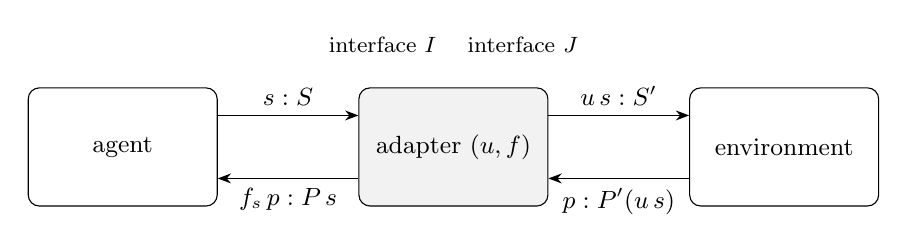
\begin{tikzpicture}[>={Stealth},font=\small]
    \node[draw,rounded corners,minimum width=2.4cm,minimum height=1.5cm] (agent) at (0,0) {agent};
    \node[draw,rounded corners,minimum width=2.4cm,minimum height=1.5cm,fill=black!5] (ad) at (4.2,0) {adapter $(u,f)$};
    \node[draw,rounded corners,minimum width=2.4cm,minimum height=1.5cm] (env) at (8.4,0) {environment};
    \draw[->] ([yshift=4mm]agent.east) -- node[above] {$s : S$} ([yshift=4mm]ad.west);
    \draw[->] ([yshift=4mm]ad.east) -- node[above] {$u\,s : S'$} ([yshift=4mm]env.west);
    \draw[<-] ([yshift=-4mm]agent.east) -- node[below] {$f_s\,p : P\,s$} ([yshift=-4mm]ad.west);
    \draw[<-] ([yshift=-4mm]ad.east) -- node[below] {$p : P'(u\,s)$} ([yshift=-4mm]env.west);
    \node[font=\footnotesize] at (4.2,1.3) {interface $I$ \hfill\quad interface $J$};
  \end{tikzpicture}
  \caption{An adapter $(u,f) : I \lens J$ translates moves forwards and responses
    backwards.  Seen from the environment, the adapted agent has interface $J$.}
  \label{fig:lens}
\end{figure}

\begin{example}\label{ex:adapters}
  (i)~\emph{Reversal of a ranking.}  A retriever exposes $k$ candidates best-first; a
  consumer expects worst-first.  The adapter is $\fn{crev}$ (Example~\ref{ex:rev}): the
  batch is re-indexed, and a response to candidate $i$ in the consumer's numbering is
  routed to candidate $k - i - 1$ in the retriever's.
  (ii)~\emph{Context window.}  An agent exposes a history of length $n$ to a model that
  accepts at most $k$ turns.  The adapter $\lastk$ has shape map
  $u\,n = \min(n,k)$ and position map $f_n\,i = i + (n \monus k)$: window position $i$
  is history position $i + (n - k)$ when $n > k$, and $i$ otherwise.
  (iii)~\emph{Fan-out and fan-in.}  An orchestrator splits a batch of $n$ requests at
  index $m$, dispatches the two parts, and reassembles the results.  Splitting is the pair
  of adapters $\fn{take}_m$, $\fn{drop}_m$; reassembly is $\app$.
\end{example}

\subsection{Agents, wrapping, and compositional verification}

\begin{definition}[Agent]\label{def:agent}
  An \emph{agent} with interface $I$ and state type $X$ is a coalgebra of the extension
  functor: a function
  \[
    a : X \to \ext{I}\,X, \qquad a\,x = (\fn{readout}\,x,\; \fn{update}\,x),
  \]
  giving, for each state, the move the agent emits and, for each possible response, the
  next state.
\end{definition}

This is the familiar notion of a Moore machine with a dependently typed input alphabet,
and it is precisely a lens $X\,y^X \to I$ in the sense of \cite{NiuSpivak24}.  Running an
agent against an environment strategy $e : \prod_{s} P\,s$ (which picks a response to
every move) produces the sequence of moves
$\fn{readout}\,x_0, \fn{readout}\,x_1, \dots$ with $x_{j+1} = \fn{update}\,x_j\,(e\,(\fn{readout}\,x_j))$
(\textsf{[Coq]} \coq{run}).

\begin{definition}[Wrapping]\label{def:wrap}
  Given an adapter $m : I \lens J$ and an agent $a : X \to \ext{I}\,X$, the
  \emph{wrapped agent} $\fn{wrap}\,m\,a : X \to \ext{J}\,X$ is $\mmap\,m \circ a$.
\end{definition}

That is, the wrapped agent emits the move $u\,(\fn{readout}\,x)$ and, on response $p$,
moves to the state $\fn{update}\,x\,(f\,(\fn{readout}\,x)\,p)$.  Three properties follow immediately from the
corresponding properties of $\mmap$; in the development they are the lemmas
\coq{wrap\_id}, \coq{wrap\_comp} and \coq{wrap\_ext\_eq}.

\begin{proposition}[Compositionality of wrapping]\label{prop:wrap}
  \leavevmode
  \begin{enumerate}[label=(\roman*),leftmargin=2em]
  \item $\fn{wrap}\,\fn{id}\,a = a$.
  \item $\fn{wrap}\,(m_2 \circ m_1)\,a = \fn{wrap}\,m_2\,(\fn{wrap}\,m_1\,a)$.
  \item If $\mmap\,m$ and $\mmap\,m'$ agree on the one-step behaviour of $a$, then
    $\fn{wrap}\,m\,a$ and $\fn{wrap}\,m'\,a$ produce the same run against every
    environment, for every number of steps.
  \end{enumerate}
\end{proposition}

Item (ii) is the ``scalability'' dividend of types described in \cite{GhaniPodcast26}:
a pipeline of adapters is itself an adapter, and it is computed on the adapters alone.
Item (iii) is the ``trustworthiness'' dividend: to establish that two wirings of a system
have the same behaviour, it suffices to establish an equation between adapters, which by
Theorem~\ref{thm:rep} is an equation between shape and position maps.  Nothing need be
known about the agent itself --- in particular nothing about the language model that may
sit inside it.  We are, with Ghani \cite{GhaniPodcast26}, verifying the plumbing, not the
engine.

\subsection{Borders and list-shaped interfaces}

An LLM produces text.  Two routes lead from text to a typed interface
\cite{GhaniPodcast26}: change the model so that it produces structured output natively,
or keep the model and parse its output against a schema at the boundary --- ``passport
control''.  The second route is what structured-output APIs \cite{OpenAIStructured24}
and tool protocols \cite{MCP24} implement today: the schema is a type, the parser is a
checker, and a parse failure is a type error caught before it propagates.  Our concern in
this paper is not the parser but what happens after it, once values of container types
are flowing between components.  Nor do we claim anything about the probabilistic
internals of the model; the agent of Definition~\ref{def:agent} is an arbitrary function
of its state.

Within that scope, the observation on which \S\ref{sec:agents-verif} rests is simple:
whenever the shape of an interface is a count --- a batch size, a window length, a number
of candidates --- the interface is list-shaped, the adapters between such interfaces are
list morphisms, and list morphisms are the subject of \S\ref{sec:arith}.

% ===========================================================================
\section{Arithmetic Verification}\label{sec:arith}
% ===========================================================================

We now turn to deciding equality between list morphisms.  We first show what a proof
looks like in the dependently typed setting (\S\ref{sec:dependent}) and why decision
procedures do not apply directly; then we derive a non-dependent representation
(\S\ref{sec:nondep}) and identify a decidable class (\S\ref{sec:presburger}).

\subsection{The dependently typed setting}\label{sec:dependent}

Consider proving that reversal is an involution.  In container terms the statement is
$(\fn{crev} \circ \fn{crev}) \eqmor \fn{id}$, and unpacking Definitions~\ref{def:comp}
and~\ref{def:eqmor} leaves two obligations:
\begin{enumerate}[leftmargin=2em]
\item $\forall n : \N.\; n = n$, for the shapes, and
\item $\forall n : \N.\, \forall i : \Fin\,n.\; \fn{rv}_n\,(\fn{rv}_n\,i) = i$, for the
  positions.
\end{enumerate}
The first is trivial and the second is a lemma about $\Fin$ proved by induction on $i$.
Appending is similar but needs more machinery.  Its container morphism is
\[
  \fn{cappn} : ((n,m) : \N \times \N \triangleleft \Fin\,n + \Fin\,m) \lens (\N \triangleleft \Fin),
  \qquad u\,(n,m) = n + m,
\]
with the reindexing map $f_{(n,m)} : \Fin(n+m) \to \Fin\,n + \Fin\,m$ reflecting the
sum structure: output positions below $n$ come from the first list and the rest from the
second.  To define $f$ one needs the injections
$\fn{finl}_{n,m} : \Fin\,n \to \Fin(n+m)$ and $\fn{finr}_{n,m} : \Fin\,m \to \Fin(n+m)$
and a non-standard eliminator for $\Fin(n + m)$ that splits an element into its $\fn{finl}$
or $\fn{finr}$ component \cite{PrinceGhaniMcBride08}.  Proofs about $\app$ then proceed
by that eliminator.

This approach captures the arithmetic of list functions elegantly, but the definitions and
eliminators are non-trivial \cite{PrinceGhaniMcBride08}, each new function may need new
ones, and --- the decisive point --- the obligations are statements about the families
$\Fin\,n$, to which arithmetic decision procedures do not apply.  If instead we could
capture the \emph{behaviour} of the dependently typed reindexing maps by functions on
$\N$, decidable arithmetic reasoning would become possible.

\subsection{Towards non-dependent representations}\label{sec:nondep}

The type $\Fin\,n$ represents the set $\{ m : \N \mid m < n \}$, and it can be translated
to and from that set:
\begin{enumerate}[leftmargin=2em]
\item $\fn{fnat} : \forall n.\, \Fin\,n \to \N$ computes the value of an element:
  $\fn{fnat}\,\fn{fz} = 0$ and $\fn{fnat}\,(\fn{fs}\,i) = S\,(\fn{fnat}\,i)$;
\item $\fn{nfin} : \forall n\,m.\, m < n \to \Fin\,n$ builds the element of value $m$
  (the case $n = 0$ is absurd, $m = 0$ gives $\fn{fz}$, and $S\,m < S\,n$ gives
  $\fn{fs}\,(\fn{nfin}\,n\,m\,\_)$ after peeling one successor off the proof);
\item $\fn{finnat} : \forall n.\, \forall i : \Fin\,n.\; \fn{fnat}\,i < n$ proves that
  values are in range.
\end{enumerate}

\begin{observation}\label{obs:one}
  Writing $\Fin\,n$ as $\{i \mid i < n\}$, a container morphism
  $(u, f) : (n : \N \triangleleft \{i \mid i < n\}) \lens (m : \N \triangleleft \{j \mid j < m\})$
  is a pair
  \[
    u : \N \to \N, \qquad f : \textstyle\prod_n\, \{i \mid i < u\,n\} \to \{j \mid j < n\},
  \]
  and an element of $\{i \mid i < n\}$ is a pair $(i, P)$ of a number $i$ and a
  \emph{proof} $P$ that $i < n$.  Equality \eqref{eq:eqmor} of two such morphisms
  $(u,f)$ and $(v,g)$ becomes
  \begin{equation}\label{eq:eqpairs}
    \inferrule{\forall n.\; u\,n = v\,n \\
               \forall n\,i\,j\,P\,Q.\; (i, P) \jmeq (j, Q) \to f\,n\,(i,P) = g\,n\,(j,Q)}
              {(u,f) = (v,g)}
  \end{equation}
  where $P : i < u\,n$ and $Q : j < v\,n$.  Note that the hypothesis
  $(i, P) \jmeq (j, Q)$ entails $i = j$; the proofs $P$ and $Q$ differ in type (one
  mentions $u$, the other $v$), which is why heterogeneous equality is still needed at
  this point.
\end{observation}

\begin{observation}\label{obs:two}
  Every reindexing map $f : \prod_n \Fin(u\,n) \to \Fin\,n$ has an \emph{arithmetic
  shadow}: a partial function on numbers, defined on $i < u\,n$, that returns the value
  of $f_n$ at the element of value $i$.  We call it $\reduce\,f$:
  \begin{equation}\label{eq:reduce}
    \reduce\,f\,n\,i\,h \;=\; \fn{fnat}\,(f_n\,(\fn{nfin}\,(u\,n)\,i\,h))
    \qquad (h : i < u\,n).
  \end{equation}
  Given the proof $h$, $\reduce\,f\,n\,i\,h$ is just a natural number, and
  $\reduce\,f$ corresponds exactly to $f$ while being stated without finite types.
  Consequently, for every $(u, f)$ there exists a total function $g : \N \times \N \to \N$
  that agrees with the shadow of $f$ wherever the latter is defined:
  \begin{equation}\label{eq:shadow}
    \forall n\,i\,(h : i < u\,n).\; g\,n\,i = \reduce\,f\,n\,i\,h .
  \end{equation}
  For reversal, $g\,n\,i = n - i - 1$, and one proves once and for all that
  $\forall n\,i\,h.\; \reduce\,\fn{rv}\,n\,i\,h = n - i - 1$.
\end{observation}

\paragraph{How the goal evolves.}  Observation~\ref{obs:two} lets us replace the second
premise of \eqref{eq:eqpairs} by arithmetic.  Suppose we have already proved $u = v$ and
are left with the position obligation.  Table~\ref{tab:goal} traces the transformation of
that obligation.

\begin{table}[t]
  \centering
  \footnotesize
  \begin{tabular}{@{}llp{6.3cm}@{}}
    \toprule
    & Goal & Step \\
    \midrule
    (a) & $\forall n\,i\,j\,P\,Q.\; (i,P) \jmeq (j,Q) \to f\,n\,(i,P) = g\,n\,(j,Q)$
        & second premise of \eqref{eq:eqpairs}, with $P : i < u\,n$, $Q : j < v\,n$ \\
    (b) & $\forall n\,i\,j\,P\,Q.\; (i,P) \jmeq (j,Q) \to \reduce\,f\,n\,i\,P = \reduce\,g\,n\,j\,Q$
        & apply $\fn{fnat}$ to both sides (it is injective) and fold
          \eqref{eq:reduce}; the elements $(i,P)$ are now written $\fn{nfin}\,(u\,n)\,i\,P$ \\
    (c) & $\forall n\,i\,j\,P\,Q.\; (i,P) \jmeq (j,Q) \to g_1\,n\,i = g_2\,n\,j$
        & rewrite with the shadow equations \eqref{eq:shadow} for $f$ and $g$ \\
    (d) & $\forall n\,i\,j\,P\,Q.\; i = j \to P \jmeq Q \to g_1\,n\,i = g_2\,n\,j$
        & decompose the pair equation, using $u\,n = v\,n$:
          $(i,P) \jmeq (j,Q) \leftrightarrow i = j \wedge P \jmeq Q$ \\
    (e) & $\forall n\,i.\; i < u\,n \to i < v\,n \to g_1\,n\,i = g_2\,n\,i$
        & substitute $j := i$; the hypothesis $P \jmeq Q$ is now vacuous (both are proofs
          of $i < u\,n$) and is discarded, leaving only the range conditions \\
    \bottomrule
  \end{tabular}
  \caption{Evolution of the position obligation.  Goal (e) mentions no finite types and
    no proofs.}\label{tab:goal}
\end{table}

The upshot is that, provided reindexing maps are given by their shadows, equality of
container morphisms between lists can be stated as
\begin{equation}\label{eq:eq16}
  \inferrule{\forall n.\; u\,n = v\,n \\
             \forall n\,i.\; i < u\,n \to i < v\,n \to g_1\,n\,i = g_2\,n\,i}
            {(u, g_1) = (v, g_2)}
\end{equation}
in place of \eqref{eq:eqmor}.  We call \eqref{eq:eq16} \emph{quasi-container} equality:
it is sound with respect to Definition~\ref{def:eqmor} (Theorem~\ref{thm:sound} below
makes this precise), but it is stated purely in arithmetic.  If $u$, $v$, $g_1$ and $g_2$
lie in a decidable fragment of arithmetic, \eqref{eq:eq16} can be decided.  Which
fragment?  The shape maps of $\fn{crev}$ (identity) and $\fn{cappn}$ (addition) suggest
linear arithmetic, and we now show that this suggestion is right.

\subsection{Presburger-definable morphisms}\label{sec:presburger}

\emph{Presburger integer arithmetic} (PIA) is the first-order theory of the structure
$\langle \Z, 0, 1, +, \le \rangle$; its restriction to the natural numbers is
\emph{Presburger natural arithmetic} (PNA).  Presburger showed that PIA is decidable
\cite{Presburger29}, and the decidability of PNA follows (interpret $\N$ as the
non-negative integers).  Cut-off subtraction and conditionals on linear inequalities are
definable in PNA: the graph of $r = a \monus b$ is
$(b \le a \wedge r + b = a) \vee (a < b \wedge r = 0)$, and the graph of
$r = (\text{if } a < b \text{ then } x \text{ else } y)$ is
$(a < b \wedge r = x) \vee (b \le a \wedge r = y)$.  We shall use this repeatedly.

\begin{definition}[Linear functions]\label{def:lfun}
  A function $F : \N^k \to \N$ is \emph{linear definable} if it is denoted by a term of
  the grammar
  \[
    \fn{lfun} \;::=\; \fn{const}\,c \;\mid\; \fn{var}\,j \;\mid\; \fn{add}\,\fn{lfun}\,\fn{lfun}
    \qquad (c \in \N,\; j < k)
  \]
  interpreted in the evident way: $\fn{const}\,c$ is the constant function,
  $\fn{var}\,j$ is the $j$-th projection and $\fn{add}$ is pointwise addition.  It is
  \emph{piecewise-linear definable} if it is denoted by a term of the extended grammar
  \[
    \fn{pl} \;::=\; \fn{lp}\,\fn{lfun}' \;\mid\; \fn{pf}\,\fn{pl}\,\fn{pl}\,\fn{pl},
    \qquad
    \fn{lfun}' \;::=\; \fn{lfun} \;\mid\; \fn{sub}\,\fn{lfun}'\,\fn{lfun}'
  \]
  where $\fn{sub}$ is cut-off subtraction and $\fn{pf}\,c\,l\,r$ denotes
  ``if $0 < c$ then $l$ else $r$''.
\end{definition}

Since a condition $a < b$ is the same as $0 < b \monus a$, nested $\fn{pf}$ expresses any
finite case analysis on linear inequalities; the grammar is that of the Coq types
\coq{lfun} and \coq{Plfun} of \S\ref{sec:coq}.  By the remarks preceding the definition,
the graph of every piecewise-linear definable function is given by a quantifier-free
formula of PNA (\textsf{[Coq]} \coq{suB\_graph}, \coq{pf\_graph}).

\begin{definition}[Linear and Presburger morphisms]\label{def:pmor}
  Let $(u, f) : (\mathbf{n} : \N^k \triangleleft \Fin\,n_1 + \dots + \Fin\,n_k) \lens (\N \triangleleft \Fin)$
  be a container morphism from $k$ lists to a list.
  \begin{enumerate}[label=(\roman*),leftmargin=2em]
  \item $(u, f)$ is \emph{linear} if $u$ is linear definable.
  \item $(u, f)$ is \emph{Presburger} if $u$ and the shadow of $f$ are piecewise-linear
    definable, where positions of the $k$ inputs are numbered consecutively, so that the
    shadow is a function $\N^k \times \N \to \N$ (output position $i$ to a position in
    $\Fin(n_1 + \dots + n_k)$).
  \end{enumerate}
\end{definition}

Cartesian morphisms are sometimes called linear in the literature
\cite{AbbottAltenkirchGhani05}; our use of ``linear'' is different (it refers to the shape
map), and we reserve ``cartesian'' for Definition~\ref{def:cartesian}.  $\fn{crev}$ and
$\fn{cappn}$ are linear, with shape maps $\fn{var}\,0$ and
$\fn{add}\,(\fn{var}\,0)\,(\fn{var}\,1)$ respectively.

\begin{proposition}\label{prop:linear-pl}
  The shadow of the reindexing map of a linear morphism is piecewise-linear definable.
\end{proposition}

\begin{proof}[Proof sketch]
  By induction on the term denoting $u$.  For $\fn{const}$ and $\fn{var}$ the shadow is
  obtained directly by $\reduce$.  For $\fn{add}\,l\,r$, an output position $i < u\,\mathbf{n}$
  satisfies either $i < l\,\mathbf{n}$ or $i - l\,\mathbf{n} < r\,\mathbf{n}$, by the lemma
  $\fn{leplus\_or} : \forall i\,n\,m.\; i < n + m \to \{i < n\} + \{i - n < m\}$; in the
  first case the position is routed through the $\fn{finl}$ component and in the second
  through the $\fn{finr}$ component, recursively.  Each split introduces one breakpoint,
  linear in the $n_j$, so the result is piecewise linear.  Full details are in
  \cite[Prop.~6.2]{Prince10}.
\end{proof}

Linear morphisms do not cover $\fn{tail}$, $\fn{head}$, $\fn{last}$ or
$\fn{but\_last}$, whose shape maps involve subtraction, nor $\fn{take}$, whose shape map is
a minimum.  All of these are Presburger morphisms, however, and in fact the Presburger
morphisms are closed under the operation that matters.

\begin{proposition}[Closure under composition]\label{prop:closure}
  If $(u_1, g_1)$ and $(u_2, g_2)$ are Presburger morphisms, so is their composite.
\end{proposition}

\begin{proof}
  By Definition~\ref{def:comp} the composite has shape map $u_2 \circ u_1$ and shadow
  $\lambda \mathbf{n}\,i.\; g_1\,\mathbf{n}\,(g_2\,(u_1\,\mathbf{n})\,i)$; piecewise-linear
  terms are closed under substitution of terms for variables, conditionals being
  propagated outwards (\textsf{[Coq]} \coq{psubst}, \coq{psubst\_ok}).
\end{proof}

\begin{theorem}[Decidability]\label{thm:decidable}
  Let $(u, g_1)$ and $(v, g_2)$ be Presburger morphisms.  The equality \eqref{eq:eq16}
  between them is decidable.  So are the \emph{range condition}
  $\forall \mathbf{n}\,i.\; i < u\,\mathbf{n} \to g_1\,\mathbf{n}\,i < n_1 + \dots + n_k$,
  and, for $k = 1$, the \emph{losslessness condition}
  \[
    \forall n.\; u\,n = n \;\wedge\; \forall i\,j.\; i < n \to j < n \to g_1\,n\,i = g_1\,n\,j \to i = j .
  \]
\end{theorem}

\begin{proof}
  Let $\gamma_u(\mathbf{n}, r)$, $\gamma_v(\mathbf{n}, r)$, $\gamma_1(\mathbf{n}, i, r)$
  and $\gamma_2(\mathbf{n}, i, r)$ be the quantifier-free PNA formulae defining the graphs
  of $u$, $v$, $g_1$ and $g_2$.  Then \eqref{eq:eq16} is equivalent to the PNA sentence
  \begin{align*}
    &\forall \mathbf{n}\,r\,r'.\; \gamma_u(\mathbf{n},r) \to \gamma_v(\mathbf{n},r') \to r = r' \\
    \wedge\;\;&\forall \mathbf{n}\,i\,r\,r_1\,r_2.\; \gamma_u(\mathbf{n},r) \to i < r \to
      \gamma_1(\mathbf{n},i,r_1) \to \gamma_2(\mathbf{n},i,r_2) \to r_1 = r_2 ,
  \end{align*}
  which is decidable by Presburger's theorem.  The other two conditions are
  translated in the same way.
\end{proof}

The proof shows more than decidability.  All three sentences are \emph{universal}: a
block of $\forall$s in front of a quantifier-free matrix.  Deciding such a sentence
amounts to deciding the unsatisfiability of a quantifier-free formula, a problem that is
NP-complete rather than doubly exponential, and that is exactly what the Omega test
\cite{Pugh91}, Coq's \coq{lia} and SMT solvers are built for.  This matters for the
practicality discussed in \S\ref{sec:coq}.  By contrast the dual of losslessness,
surjectivity of the position maps ($\forall n\,j.\, j < n \to \exists i < u\,n.\, g_1\,n\,i = j$),
has an existential quantifier and lies outside the fragment; happily, for finite sets
injectivity together with $u\,n = n$ already implies bijectivity, which is why the
losslessness condition is stated as it is.

\subsection{Representing Presburger morphisms}\label{sec:ppcm}

We now fix the concrete representation used in the development.  A Presburger morphism
of \emph{arity} $k$ (from $k$ lists to a list) is a pair of piecewise-linear terms
\[
  \mathsf{PPCm} \;=\; \fn{pl} \times \fn{pl},
\]
the first denoting the shape map over the variables $0, \dots, k-1$ (the input lengths),
the second denoting the shadow over the variables $0, \dots, k$, where variable $k$ is the
output position $i$.  Positions of the $k$ inputs are numbered consecutively (``flat''
encoding), via the isomorphism $\Fin\,n_1 + \dots + \Fin\,n_k \cong \Fin(n_1 + \dots + n_k)$.

\begin{example}\label{ex:ppcm}
  Writing $x_0, x_1, x_2$ for the variables,
  \begin{align*}
    \fn{Rev} &= (x_0,\; (x_0 \monus x_1) \monus 1) &
    \fn{Tail} &= (x_0 \monus 1,\; x_1 + 1) \\
    \fn{Take}_m &= (\text{if } x_0 < m \text{ then } x_0 \text{ else } m,\; x_1) &
    \fn{Drop}_m &= (x_0 \monus m,\; x_1 + m) \\
    \fn{App} &= (x_0 + x_1,\; x_2) &
    \lastk &= (\text{if } x_0 < k \text{ then } x_0 \text{ else } k,\; x_1 + (x_0 \monus k)).
  \end{align*}
  Observe that with the flat encoding the position map of $\fn{App}$ is the identity: output
  position $i$ is input position $i$ of the concatenation.\footnote{The 2011 version of this paper
  and its code gave a position map that subtracted $n$ in the second case, which double
  counts the offset that the interpretation already applies; see \S\ref{sec:coq}.}
\end{example}

The \emph{interpretation} of $(u, g) : \mathsf{PPCm}$ of arity $k$ on inputs
$(n_1, h_1), \dots, (n_k, h_k)$, where $h_j : \N \to X$ is the lookup function of the $j$-th
list, is
\begin{equation}\label{eq:interp}
  \llbracket (u,g) \rrbracket\, \big((n_1,h_1),\dots,(n_k,h_k)\big) \;=\;
  \big(u\,\mathbf{n},\; \lambda i.\; \fn{flat}\,(g\,\mathbf{n}\,i)\big),
\end{equation}
where $\fn{flat}\,p = h_1\,p$ if $p < n_1$, $\fn{flat}\,p = h_2\,(p - n_1)$ if
$n_1 \le p < n_1 + n_2$, and so on (\textsf{[Coq]} \coq{interp}, \coq{flat}).  This is
$\mmap$ of \eqref{eq:mmap} for the flat encoding; a default value is returned for an
out-of-range position, which a morphism satisfying the range condition of
Theorem~\ref{thm:decidable} never produces.

\begin{theorem}[Soundness of quasi-container equality]\label{thm:sound}
  \textsf{[Coq: \coq{pcmEQ\_ok}]}  If $(u, g_1)$ and $(v, g_2)$ satisfy \eqref{eq:eq16},
  then for all inputs their interpretations have the same length and the same element at
  every position.
\end{theorem}

\begin{definition}[Composition of representations]\label{def:ppcomp}
  Let $l = (u_l, g_l)$ have arity $1$ and $r = (u_r, g_r)$ have arity $k$.  Their
  composite $\fn{comp}_1\,l\,r$, of arity $k$, is
  \[
    \big(\; u_l[x_0 := u_r],\;\; g_r[x_k := g_l[x_0 := u_r,\, x_1 := x_k]] \;\big),
  \]
  where $t[x := s]$ is substitution of piecewise-linear terms.  Let $l$ have arity $2$ and
  $r_1 = (u_1, g_1)$, $r_2 = (u_2, g_2)$ have arity $k$ \emph{over the same $k$ inputs}.
  Their composite $\fn{comp}_2\,l\,r_1\,r_2$, of arity $k$, has shape map
  $u_l[x_0 := u_1, x_1 := u_2]$ and, with $q = g_l[x_0 := u_1, x_1 := u_2, x_2 := x_k]$
  the position in the intermediate concatenation, position map
  \[
    \text{if } q < u_1 \text{ then } g_1[x_k := q] \text{ else } g_2[x_k := q \monus u_1] .
  \]
\end{definition}

The first clause is Definition~\ref{def:comp} written out for terms.  The second is the
composition needed for a binary function applied to two functions of the same argument(s)
--- for instance $\fn{take}_m\,b \app \fn{drop}_m\,b$, or $\rev\,ys \app \rev\,xs$ as a
function of $(xs, ys)$ --- and it is where the flat encoding earns its keep: the position
map is a case split on which intermediate list the position falls in.  (In the
development the terms substituted for $u_r$, $u_1$, $u_2$ are first \emph{shielded}, that
is, their variables $\ge k$ are set to $0$, so that a term of arity $k$ cannot observe the
output-position variable of the composite; this makes the following theorem exact rather
than subject to a free-variable side condition.)

\begin{theorem}[Correctness of composition]\label{thm:comp}
  \textsf{[Coq: \coq{comp1\_ok}, \coq{comp2\_ok}]}
  If $l$ satisfies the range condition, then for all inputs $\mathbf{x}$,
  \begin{align*}
    \llbracket \fn{comp}_1\,l\,r \rrbracket\,\mathbf{x} &= \llbracket l \rrbracket\,(\llbracket r \rrbracket\,\mathbf{x}) \\
    \llbracket \fn{comp}_2\,l\,r_1\,r_2 \rrbracket\,\mathbf{x} &= \llbracket l \rrbracket\,(\llbracket r_1 \rrbracket\,\mathbf{x}, \llbracket r_2 \rrbracket\,\mathbf{x}),
  \end{align*}
  up to equality of lengths and of elements at every position.
\end{theorem}

Equality \eqref{eq:eq16} is implemented as a proposition \coq{pcmEQ} and decided by the
tactic \coq{containers} described in \S\ref{sec:coq}.

\subsection{A closer look at some functions}\label{sec:closer}

The shape map of a function in this setting is exactly the shape map of its container
morphism, while its position map is the shadow of the container morphism's reindexing
map.  To represent a function one therefore states what its container morphism does to
lengths and indices, and the representation can usually be read off a whiteboard.

\paragraph{\fn{take} and \fn{drop}.}  $\fn{take}_m$ retains the first $m$ elements: if
$m < n$ the output has length $m$, otherwise $n$, and output position $i$ is always input
position $i$.  $\fn{drop}_m$ removes the first $m$ elements: the output has length
$n \monus m$ and output position $i$ is input position $i + m$.  Hence the representations
in Example~\ref{ex:ppcm}.  Note that $\fn{take}_m$ is \emph{not} cartesian: when $m < n$
positions $m, \dots, n-1$ of the input are dropped.

\paragraph{\fn{head}, \fn{last}, \fn{but\_last} and \fn{tail}.}  As functions
$\List\,X \to \List\,X$ (returning a list of length at most one, to stay polymorphic),
$\fn{head}$ and $\fn{last}$ have shape map $n \monus (n \monus 1)$, which is $1$ for $n > 0$
and $0$ for $n = 0$; the single output position is input position $0$ for $\fn{head}$ and
$n - 1$ for $\fn{last}$.  $\fn{but\_last}$ has shape map $n \monus 1$ and identity position
map; $\fn{tail}$ has the same shape map and position map $i + 1$.

\paragraph{Rotation.}  $\fn{rot}$ moves the first element to the back and
$\fn{unrot}$ moves the last element to the front.  Both keep the length.  Output position
$i$ of $\fn{rot}$ is input position $i + 1$ when $i < n - 1$ and $0$ otherwise; output
position $i$ of $\fn{unrot}$ is input position $i - 1$ when $i > 0$ and $n - 1$ otherwise.
In the dependently typed representation these require the view of $\Fin(S\,n)$ as
$\fn{top}$-or-$\fn{emb}$ (Example~\ref{ex:rev}); here they are two conditionals.

\begin{figure}[t]
  \centering
  \begin{minipage}{0.48\textwidth}
    \begin{align*}
      \rev\,(\rev\,xs) &= xs \\
      \rev\,(xs \app ys) &= \rev\,ys \app \rev\,xs \\
      \fn{head}\,(\rev\,xs) &= \fn{last}\,xs \\
      \fn{tail}\,(\rev\,xs) &= \rev\,(\fn{but\_last}\,xs) \\
      \fn{drop}_n\,(\fn{drop}_m\,xs) &= \fn{drop}_{n+m}\,xs \\
      \fn{drop}_n\,(\fn{take}_m\,xs) &= \fn{take}_{m-n}\,(\fn{drop}_n\,xs) \\
      \fn{take}_n\,(\fn{drop}_m\,xs) &= \fn{drop}_m\,(\fn{take}_{n+m}\,xs)
    \end{align*}
  \end{minipage}
  \begin{minipage}{0.48\textwidth}
    \begin{align*}
      \fn{drop}_1\,(\fn{unrot}\,xs) &= \fn{but\_last}\,xs \\
      \fn{rot}\,(\fn{unrot}\,xs) &= xs \\
      \fn{unrot}\,(\fn{rot}\,xs) &= xs \\
      \fn{head}\,(\rev\,(\fn{rot}\,xs)) &= \fn{head}\,xs \\
      \fn{last}\,(\fn{rot}\,xs) &= \fn{head}\,xs \\
      \fn{head}\,(\fn{unrot}\,xs) &= \fn{last}\,xs \\
      \fn{but\_last}\,(\fn{rot}\,xs) &= \fn{tail}\,xs
    \end{align*}
  \end{minipage}
  \caption{Properties of lists proved automatically by the tactic \coq{containers}
    (\textsf{[Coq]} file \coq{Examples.v}).  Each is stated as a \coq{pcmEQ} between
    composites of the representations of Example~\ref{ex:ppcm}.}\label{fig:properties}
\end{figure}

Figure~\ref{fig:properties} lists properties that are proved automatically.  Several
of them were beyond the scope of the ellipsis technique \cite{BundyRichardson99,Prince05},
and all of them are proved without the subsidiary lemmas and eliminators that the
dependently typed system of \cite{PrinceGhaniMcBride08} required.

\subsection{The Coq development}\label{sec:coq}

The updated development consists of four
files, compiles with Coq 8.18 and the Rocq Prover, uses only the standard library, and
contains no axioms or admitted lemmas.

\paragraph{\coq{Piecewise.v}.}  The grammar of Definition~\ref{def:lfun} is the pair of
inductive types
\begin{lstlisting}
Inductive lfun : Set :=                  Inductive Plfun : Set :=
  | cnst : nat -> lfun                     | lp : lfun -> Plfun
  | vr   : nat -> lfun                     | pf : Plfun -> Plfun -> Plfun -> Plfun.
  | adD  : lfun -> lfun -> lfun
  | suB  : lfun -> lfun -> lfun.
\end{lstlisting}
with evaluation functions \coq{evl} and \coq{pevl} against an environment
$\rho : \N \to \N$ (variable $j$ reads $\rho\,j$).  Variables are plain numbers rather
than elements of \coq{Fin n}, which removes every dependent pattern match from the
arithmetic core.  Substitution \coq{psubst} is defined with conditionals propagated
outwards, and proved correct.

\paragraph{\coq{ListMorphisms.v}.}  A morphism is a pair \coq{PPCm := Plfun * Plfun};
its arity is supplied to the equality and the interpretation rather than carried in the
type.  The file defines the interpretation \eqref{eq:interp}, the equality
\begin{lstlisting}
Definition pcmEQ (k : nat) (l r : PPCm) : Prop :=
  forall rho, pevl (shape l) rho = pevl (shape r) rho /\
    forall i, i < pevl (shape l) rho ->
      pevl (pos l) (ext rho k i) = pevl (pos r) (ext rho k i).
\end{lstlisting}
(where \coq{ext rho k i} binds variable $k$ to $i$), its soundness
(Theorem~\ref{thm:sound}), the range and losslessness conditions, composition
(Definition~\ref{def:ppcomp}) with its correctness (Theorem~\ref{thm:comp}), and the tactic
\begin{lstlisting}
Ltac containers := unfold_morphism; arith.
\end{lstlisting}
Here \coq{unfold\_morphism} unfolds the definitions, splits the conjunction, evaluates the
terms symbolically (rewriting with the correctness lemmas for substitution) and
\coq{arith} eliminates every remaining conditional by case analysis and calls \coq{lia}.
The \coq{optimiseOmega} pre-processing of the 2011 tactic, which discarded redundant
hypotheses and performed ad hoc inequality reasoning to help \coq{omega}, is no longer
needed.

\paragraph{\coq{Examples.v}.}  The representations of Example~\ref{ex:ppcm} and the
properties of Figure~\ref{fig:properties}, each proved by \coq{containers}.  Two
definitions of the 2011 code were found, in preparing this revision, to be wrong:
\coq{take1} had shape map $\max(n,m)$ rather than $\min(n,m)$ (a swapped conditional), and
\coq{appn1}'s position map did not follow the flat encoding of the interpretation.  The
2011 lemmas about them were therefore theorems about the wrong functions.  Both are
corrected, the properties are re-proved, and each basic morphism is now validated against
the standard library by a \emph{transfer lemma}, e.g.
\begin{lstlisting}
Lemma Take_spec : forall m (l : list X),
    RepEq (interp (Take m) [of_list d l] d) (of_list d (firstn m l)).
\end{lstlisting}
where \coq{of\_list} turns a list into a length-and-lookup pair and \coq{RepEq} is equality
of length and of elements at every position.  These lemmas answer a question put by one of
the referees: how hard is it to relate the container-style definitions to the usual
recursive ones?  Each transfer lemma is a short structural induction (between three and
ten lines; \coq{Rev\_spec} uses the library lemma \coq{rev\_nth}), and it is done once per
function, not once per property.  With the transfer lemmas in hand, theorems about
ordinary lists follow from the decision procedure \emph{with no induction at all}: the
file derives, among others,
\begin{lstlisting}
Theorem rev_involutive_via_containers : forall l : list X, rev (rev l) = l.
Theorem firstn_skipn_via_containers : forall m (l : list X), firstn m l ++ skipn m l = l.
\end{lstlisting}
by chaining the transfer lemmas, Theorem~\ref{thm:comp}, Theorem~\ref{thm:sound} and the
relevant \coq{pcmEQ}.  This is the ``two-tier'' methodology the referee suggested: one
recursive definition per function for programming, one container representation per
function for proving, connected once.

\paragraph{\coq{Containers.v}.}  Containers, extensions, morphisms, $\mmap$ with its
functoriality, cartesian morphisms, agents, wrapping and runs, exactly as in
\S\ref{sec:containers}--\ref{sec:agents}; and the bridge to the arithmetic
representation described in \S\ref{sec:agents-verif}.

\paragraph{Performance.}  Table~\ref{tab:perf} compares proof times.  The original development
took 6\,s for $\rev \circ \rev = \fn{id}$ on the machine of \cite{Prince10}. % and one referee
%measured 75\,s for one of the examples on a contemporary Intel i5 (and did not see it
%finish in 30 minutes on an older machine).  
The new development proves every property of
Figure~\ref{fig:properties} in at most 0.2\,s (all but one in under 40\,ms), and the most expensive statement in the
development (the sliding-window invariant of \S\ref{sec:agents-verif}, which composes an
arity-2 morphism) in 0.43\,s.  Three things account for the difference: \coq{lia}
(Micromega) replaces \coq{omega}, which was deprecated in Coq 8.12 and removed in 8.14;
the non-dependent, nat-indexed terms give \coq{lia} small goals with few atoms; and the
universal form of the statements (Theorem~\ref{thm:decidable}) puts them in the
quantifier-free fragment for which these procedures are designed.

\begin{table}[t]
  \centering\small
  \begin{tabular}{@{}lrr@{}}
    \toprule
    Statement & 2011 code  & this version \\ %& 2014 referee
    \midrule
    $\rev\,(\rev\,xs) = xs$  & 6\,s & 0.02\,s \\ %& 6\,s
    $\fn{take}_n\,(\fn{drop}_m\,xs) = \fn{drop}_m\,(\fn{take}_{n+m}\,xs)$  & --- & 0.02\,s \\ %& ---
    $\fn{head}\,(\rev\,(\fn{rot}\,xs)) = \fn{head}\,xs$ & --- & 0.04\,s \\ %& --- 
    $\rev\,(xs \app ys) = \rev\,ys \app \rev\,xs$ & not provable$^\dagger$  & 0.18\,s \\ %& ---
    $\fn{take}_m\,b \app \fn{drop}_m\,b = b$  & --- & 0.06\,s \\ %& ---
    $\lastk\,(h \app t) = \lastk\,(\lastk\,h \app t)$  & --- & 0.43\,s \\ %& ---
   % ``one of the enclosed examples'' & --- & 75\,s & $\le 0.43$\,s \\
    \bottomrule
  \end{tabular}
  \caption{Time taken by the tactic (Coq 8.18, Intel Xeon 2.1\,GHz).  The 2011 figure is
    from \cite[\S6.3.2]{Prince10} (Intel E5200).  $^\dagger$The 2011 code could not state this property, lacking the
    composition $\fn{comp}_2$.}\label{tab:perf}
\end{table}

\paragraph{Limitations.}  The procedure handles polymorphic functions
$\List(X)^k \to \List(X)$ whose container morphisms are Presburger.  Functions on nested
lists, and functions into other data types, are outside its scope; \S\ref{sec:conclusion}
discusses extensions.

% ===========================================================================
\section{Verifying List-Shaped Agent Adapters}\label{sec:agents-verif}
% ===========================================================================

We now combine \S\ref{sec:agents} and \S\ref{sec:arith}.  Throughout, ``adapter'' means
an adapter between list-shaped interfaces, represented as in \S\ref{sec:ppcm}.

\subsection{From arithmetic equality to agent behaviour}

The arithmetic representation lives on natural numbers; the agents of
Definition~\ref{def:agent} live on the list container with its dependently typed
positions.  The two are connected by the range condition.

\begin{theorem}\label{thm:bridge}
  \textsf{[Coq: \coq{to\_cmor}, \coq{to\_cmor\_interp}, \coq{pcmEQ\_wrap}]}
  \leavevmode
  \begin{enumerate}[label=(\roman*),leftmargin=2em]
  \item Every representation $m = (u, g)$ of arity $1$ satisfying the range condition
    determines a container morphism $\widehat{m} : (\N \triangleleft \Fin) \lens (\N \triangleleft \Fin)$,
    with shape map $u$ and position map $f_n\,i = g\,n\,i$ (the range condition supplies
    the proof that $g\,n\,i < n$).
  \item The extension of $\widehat{m}$ agrees with the interpretation
    \eqref{eq:interp} of $m$: reading a list off $\mmap\,\widehat{m}\,e$ gives the same
    length and elements as applying $\llbracket m \rrbracket$ to the list read off $e$.
  \item Consequently, if $l$ and $r$ satisfy the range condition and
    $\fn{pcmEQ}\,l\,r$ holds, then for every agent $a$ on the list interface and every
    state $x$, the one-step behaviours $\fn{wrap}\,\widehat{l}\,a\,x$ and
    $\fn{wrap}\,\widehat{r}\,a\,x$ have the same move and the same continuation at every
    response; by Proposition~\ref{prop:wrap}(iii) the wrapped agents have the same runs.
  \end{enumerate}
\end{theorem}

Part (iii) is the statement that an equation decided by \coq{containers} is a theorem
about \emph{behaviour}: whatever the agent --- an LLM-backed planner, a retriever, a
hand-written state machine --- the two adapters make it indistinguishable to its
environment.

\subsection{Losslessness}

An adapter that drops or duplicates responses is sometimes intended ($\lastk$ must drop
old turns) and sometimes a bug (a fan-in that loses a tool result).  Either way it is a
fact worth knowing, and for governance and auditability it is a fact worth
\emph{checking}.

\begin{proposition}\label{prop:lossless}
  \textsf{[Coq: \coq{lossless} and the lemmas \coq{*\_lossless}, \coq{*\_lossy}]}
  Losslessness of an adapter --- cartesianness of the corresponding container morphism
  --- is decidable (Theorem~\ref{thm:decidable}).  Reversal and the two rotations are
  lossless; $\fn{tail}$, $\fn{take}_m$, $\fn{drop}_{m+1}$ and $\lastk$ are not, and the
  procedure exhibits a witness in each case (a history of length $k + 1$ for $\lastk$).
\end{proposition}

\subsection{Worked examples}\label{sec:worked}

All statements in this section are from the file \coq{Examples.v}, where each is proved
or refuted by the tactic \coq{containers} in well under a second.

\paragraph{Context windows.}  Let $h$ be a history and $t$ the new turns to be appended.
A sliding-window implementation must decide whether to truncate before or after
appending.  The procedure proves that it does not matter:
\begin{equation}\label{eq:window}
  \lastk\,(h \app t) \;=\; \lastk\,(\lastk\,h \app t),
\end{equation}
so a system may keep only the last $k$ turns between calls without ever diverging from a
system that keeps everything and truncates on demand.  In the representation,
\eqref{eq:window} is the equality of arity-2 morphisms
\[
  \fn{comp}_1\,\lastk\,\fn{App} \;=\; \fn{comp}_1\,\lastk\,\big(\fn{comp}_2\,\fn{App}\,(\lastk \text{ on } x_0)\,(\fn{id} \text{ on } x_1)\big)
\]
(\textsf{[Coq]} \coq{lastk\_app}).  Two further
invariants are proved in the same way: truncation is idempotent,
$\lastk\,(\lastk\,h) = \lastk\,h$, and nested windows collapse to the tighter one,
$\lastk\,(\fn{last}_{k+1}\,h) = \lastk\,h$.

\paragraph{A refuted law.}  It is tempting to ``optimise'' the window by dropping the
oldest turn of a $(k+1)$-window, on the grounds that
$\fn{drop}_1\,(\fn{last}_{k+1}\,h) = \lastk\,h$.  This is false when the history is shorter
than the window: for a history of length $1$ and $k = 1$ the left side is empty and the
right side is not.  The procedure refutes it with exactly that witness (\textsf{[Coq]}
\coq{drop\_lastk\_refuted}).  Likewise an off-by-one position map,
$f_n\,i = i + (n \monus k) + 1$, is rejected with the witness $n = k + 1$, $i = 0$
(\coq{badlastk\_detected}).  A false adapter law is a routing bug: the agent would be
shown the wrong turn.  That the same procedure both proves the true laws and refutes the
false ones with counterexamples is, for this application, the essential property.

\paragraph{Fan-out and fan-in.}  An orchestrator that splits a batch of $n$ requests at
index $m$ and reassembles the $n$ results must restore the original correspondence between
requests and results.  The procedure proves
$\fn{take}_m\,b \app \fn{drop}_m\,b = b$ as an equation between the arity-1 morphisms
$\fn{comp}_2\,\fn{App}\,\fn{Take}_m\,\fn{Drop}_m$ and $\fn{id}$
(\textsf{[Coq]} \coq{split\_merge}): result $i$ is routed back to request $i$.  Together
with Proposition~\ref{prop:wrap}(ii) this scales: a tree of splits and merges is a
composite of adapters, and its equality to the identity is one \coq{pcmEQ}.

\paragraph{Reorderings.}  The identities of Figure~\ref{fig:properties} read, in the
agent setting, as facts about rankings and histories: ``the top candidate of the reversed
ranking is the bottom candidate of the original'' ($\fn{head} \circ \rev = \fn{last}$),
``reversing twice is the identity'', ``rotating a round-robin schedule forward and then
back changes nothing'' ($\fn{unrot} \circ \fn{rot} = \fn{id}$).

\subsection{Generate and check}\label{sec:generate-check}

It would be interesting to consider whether the translation from a recursive definition to its container
representation could be automated. %, calling it a potential ``game changer''.
Two developments since 2011 bear on this.  First, the thesis \cite[\S7.2.3]{Prince10} already
gives a \emph{semantic} translation: for any polymorphic $F : \forall X.\, \List\,X \to \List\,X$,
Theorem~\ref{thm:rep} yields its container morphism, and $\reduce$ \eqref{eq:reduce}
yields the shadow; what is not automatic is recognising the shadow as a piecewise-linear
\emph{term}, which is a normalisation problem rather than a proof problem.  Second, the
division of labour between an untrusted \emph{proposer} and a trusted \emph{checker} has
become the standard architecture for combining language models with proof assistants
\cite{Harmonic25,AlphaProof24}, and it fits here exactly: a model may propose the
representation $(u, g)$ of a function together with its transfer lemma, and the
transfer lemma's proof (a short induction) and all subsequent properties (decided by
\coq{containers}) are checked by Coq.  Ghani's remark that a language model is ``like a
precocious PhD student'' who ``talks nonsense quite often'' \cite{GhaniPodcast26} is
precisely the reason the checker must be a decision procedure and not another model.  
%The referee's other concern, that index arithmetic is an unnatural way to program, is in this
Correspondingly, the concern at the time the originaly work appeared that index arithmetic 
is an unnatural way to program, is in this domain inverted: index arithmetic on histories and batches
(\texttt{history[-k:]}, \texttt{results[i]}) is how orchestration code is written today.
What is missing is the proof that the arithmetic is right, which is what the procedure
supplies.

\subsection{What this does and does not establish}

The results above are about the composition of components along typed, list-shaped
interfaces.  They say nothing about whether a language model will produce a parseable
output (that is the parser's job), nothing about the model's internals, and nothing about
interfaces whose shape is not a count.  Within their scope they deliver, for the list
fragment, the three properties that Kodamai's ``math-first'' programme asks of enterprise
agents \cite{KodamaiEEJ26}: adapters are verified rather than tested (``error-proof''),
interfaces are typed contracts specific to the data flowing through them
(``specialised''), and a component can be swapped for another with the same interface,
with the equations between adapters guaranteeing that the swap is behaviour-preserving
(``adaptive'').  Extending the decidable fragment beyond lists --- to trees, to interfaces
indexed by several counts, to the mode-dependent interfaces of \cite{Spivak26} --- is the
natural next step, and \S\ref{sec:conclusion} outlines it.

% ===========================================================================
\section{Related Work}\label{sec:related}
% ===========================================================================

\paragraph{Containers and polynomial functors.}  Containers were introduced by Abbott,
Altenkirch and Ghani \cite{Abbott03,AbbottAltenkirchGhani03,AbbottAltenkirchGhani05} as a
semantic account of strictly positive data types, and extended to indexed containers in
\cite{AltenkirchGhaniHancockMcBrideMorris15}.  Polynomial functors, the same objects in a
categorical dress, were studied by Gambino and Kock \cite{GambinoKock13} and taken up by
Spivak as a setting for ``mode-dependent dynamics'' \cite{Spivak20}; the monograph of Niu
and Spivak \cite{NiuSpivak24} develops the category $\Poly$ systematically, including the
reading of lenses as interfaces of interacting systems that \S\ref{sec:agents} adopts.
Libkind and Spivak \cite{LibkindSpivak24} use polynomial functors to model hierarchical
task delegation between agents, with morphisms as delegations; our adapters are the
special case of list-shaped interfaces, and our contribution is the decision procedure
for that case.  Spivak's recent work on interfaces that change during interaction
\cite{Spivak26} suggests where a richer decidable fragment might be sought.  Lenses as
bidirectional transformations go back to the view-update problem; their use in
compositional game theory \cite{GhaniHedgesWinschelZahn18} and categorical cybernetics
\cite{CapucciGavranovicHedgesRischel22} is the nearest precedent for ``adapters that route
information backwards''.

\paragraph{Containers in reasoning.}  Containers were used to construct polymorphic
programs with quotient types in \cite{AbbottAltenkirchGhaniMcBride04}, and as the
underpinning of the ellipsis technique in \cite{PrinceGhaniMcBride08}, of which the
present paper is a continuation.  Generic programming with containers and universes is
treated in \cite{AltenkirchMcBrideMorris07,Morris07}.

\paragraph{Typed agentic AI.}  The gap between untyped LLM output and typed components is
addressed in practice by structured-output APIs that constrain generation to a JSON schema
\cite{OpenAIStructured24} and by tool protocols such as the Model Context Protocol
\cite{MCP24}, which type tool invocations and results.  Kodamai's Calvin Grove platform
\cite{KodamaiEEJ26} composes agents as typed microservices whose interfaces are
``contracts'', with the stated aim of correctness by construction; Ghani describes its
type system as built on containers, with agents as first-class values that can be passed
to and returned by other agents \cite{GhaniPodcast26}.  The present paper supplies a
decision procedure for one fragment of such a type system.  On the proof side, Harmonic's
Aristotle \cite{Harmonic25} and DeepMind's AlphaProof \cite{AlphaProof24} produce
Lean proofs checked by the kernel; \S\ref{sec:generate-check} places our procedure in the
same proposer/checker architecture.

\paragraph{Decision procedures for data structures.}  Suter, Dotta and Kuncak
\cite{SuterDottaKuncak10} extend quantifier-free constraints on algebraic data types with
catamorphisms, allowing reasoning about the relationship between a data structure and the
value of a recursive function applied to it.  Zhang, Sipma and Manna \cite{ZhangSipmaManna04}
combine recursive data structures with Presburger arithmetic through size functions.
Bouajjani et al.\ \cite{BouajjaniDrEnSi09} define a logic for composite data structures
with a decidable satisfiability problem.  Ghilardi et al.\ \cite{GhilardiNRZ07} extend the
theory of arrays with Presburger-definable indices; Bradley, Manna and Sipma
\cite{BradleyMannaSipma06} identify a decidable fragment of the theory of arrays,
extended to infinite arrays by Habermehl, Iosif and Vojnar \cite{HabermehlIosifVojnar08}
using automata \cite{Buchi60}.  Arons et al.\ \cite{AronsPRXZ01} verify parameterized systems
by automatically computed inductive assertions.  Our procedure differs from all of these in
its object: not the values stored in a structure but the \emph{polymorphic} functions
between structures, obtained through the representation theorem; the arithmetic is on
lengths and indices alone.

\paragraph{Presburger arithmetic in verification.}  Presburger's theorem \cite{Presburger29}
and its rational analogue \cite{KreiselKrivine67} underlie a large number of tools.  The
Omega test \cite{Pugh91} has been used for timing verification \cite{AmonBHL97} and
datapath verification \cite{BrinkmannDrechsler02,JohannsenDrechsler01}.  In proof
assistants, Coq's \coq{omega} has been superseded by the certificate-checking \coq{lia}
of the Micromega plugin, and Lean~4 acquired an \coq{omega} decision procedure in 2024
\cite{Lean470}; the procedure of this paper is independent of the choice and would port to
Lean directly.  The canonical form for piecewise-linear functions of Chua and Kang
\cite{ChuaKang77}, used in \cite[Ch.~5]{Prince10} to decide equality of piecewise-linear
functions over ordered fields, is not needed here because the statements of
Theorem~\ref{thm:decidable} are handled directly by the arithmetic procedure; Carette
\cite{Carette07} gives canonical forms for more general piecewise functions.

% ===========================================================================
\section{Conclusion and Further Work}\label{sec:conclusion}
% ===========================================================================

We have shown how the container representation of polymorphic functions between lists can
be reduced to arithmetic on natural numbers, how equality of such functions becomes a
universal sentence of Presburger arithmetic when the shape and position maps are
piecewise linear, and how the resulting decision procedure proves the usual identities
between list functions without induction.  We have then read the same mathematics as a
theory of typed agent interfaces: container morphisms are adapters, wrapping is
functorial, and for list-shaped interfaces the equality and losslessness of adapters are
decidable, with behavioural consequences for every agent so wrapped.  The accompanying
development is new, axiom-free, and fast.

Several directions remain.

\paragraph{Nested lists and other data types.}  The procedure handles
$\List(X)^k \to \List(X)$ only.  For nested lists the shape of the inner lists is a vector
of lengths; extending the term language so that $\fn{var}$ ranges over a vector of
vectors is straightforward syntactically, but the resulting position maps need
quantification over the inner index and may leave the universal fragment.  For other data
types a promising starting point is the data types with a \emph{cartesian} morphism into
lists.  The function that flattens a binary tree into a list is one: for each tree shape
$s$ its position map $\Fin(\fn{Sum}\,s) \to \fn{nodes}\,s$ is a bijection, so no datum is
lost or duplicated. % (One referee objected that flattening is not injective on trees, and
%gave two binary search trees with different shapes and the same flattening; the
%observation is correct, but it concerns the \emph{shape} map, which cartesianness does not
%constrain.  A cartesian morphism may merge shapes; it may not lose positions.)  
Through such a morphism, reindexing maps between trees may be representable as 
reindexing maps between lists, and hence decided.

\paragraph{Full Presburger arithmetic.}  Properties with existential content ---
surjectivity of a position map, or the existence of a split point with some property ---
leave the universal fragment.  They remain decidable, by Cooper's algorithm or by
automata-based procedures, at a higher cost.  An implementation along the lines of
\cite{HabermehlIosifVojnar08} would extend the range of adapter properties that can be
checked.

\paragraph{Higher-order adapters.}  $\Poly$ is monoidal closed \cite{NiuSpivak24}, so the
adapters between two interfaces form an interface $[I, J]$, and ``meta-agents'' that take
agents as inputs and return agents \cite{GhaniPodcast26} are agents on such interfaces.
Our procedure decides equality in the list-shaped, Presburger fragment of $[I, J]$; a
natural question is whether a decidable fragment of the full internal hom can be
identified, which would make the typing of meta-agents checkable rather than merely
expressible.

\paragraph{Mode-dependent interfaces.}  Interfaces whose positions depend on the
history of the interaction \cite{Spivak26} are the general case of a context window: the
window's shape at step $t$ depends on everything emitted so far.  The window invariants of
\S\ref{sec:worked} are the first examples of equations between such interfaces that can be
decided; characterising the decidable fragment is open.

\paragraph{Portability.}  Nothing in the development depends on Coq specifically.  A Lean~4
port, using its \coq{omega} tactic, would bring the procedure to the proof assistant in
which most LLM-generated proofs are currently checked.

\section*{Acknowledgements}

I am grateful to Neil Ghani for suggesting, fifteen years after the fact, that this work
be revisited in the light of agentic AI, and for the conversations that shaped
\S\ref{sec:agents}; to Thorsten Altenkirch and Conor McBride for their part in the original
work; and to the two anonymous referees of the 2011 submission, whose detailed reports
are addressed point by point in the revision.
%\todo{Rawle: journals increasingly require a statement on the use of AI tools in preparing
%a manuscript; the revision was drafted with the assistance of an AI model and then
%checked by the author --- decide whether and how to state this.}

% ===========================================================================
\begin{thebibliography}{99}
\small

\bibitem{Abbott03} M.~Abbott.  \emph{Categories of Containers}.  Ph.D.\ thesis, University of Leicester, 2003.

\bibitem{AbbottAltenkirchGhani03} M.~Abbott, T.~Altenkirch and N.~Ghani.  Categories of containers.  In A.~Gordon (ed.), \emph{Proceedings of FOSSACS 2003}, LNCS 2620, pp.~23--38.  Springer, 2003.

\bibitem{AbbottAltenkirchGhani05} M.~Abbott, T.~Altenkirch and N.~Ghani.  Containers: constructing strictly positive types.  \emph{Theoretical Computer Science} 342(1):3--27, 2005.

\bibitem{AbbottAltenkirchGhaniMcBride04} M.~Abbott, T.~Altenkirch, N.~Ghani and C.~McBride.  Constructing polymorphic programs with quotient types.  In \emph{Mathematics of Program Construction (MPC 2004)}, LNCS 3125.  Springer, 2004.

\bibitem{AlphaProof24} AlphaProof and AlphaGeometry teams.  AI achieves silver-medal standard solving International Mathematical Olympiad problems.  Google DeepMind, July 2024.

\bibitem{AltenkirchGhaniHancockMcBrideMorris15} T.~Altenkirch, N.~Ghani, P.~Hancock, C.~McBride and P.~Morris.  Indexed containers.  \emph{Journal of Functional Programming} 25, e5, 2015.

\bibitem{AltenkirchMcBrideMorris07} T.~Altenkirch, C.~McBride and P.~Morris.  Generic programming with dependent types.  In \emph{Datatype-Generic Programming}, LNCS 4719, pp.~209--257.  Springer, 2007.

\bibitem{AmonBHL97} T.~Amon, G.~Borriello, T.~Hu and J.~Liu.  Symbolic timing verification of timing diagrams using Presburger formulas.  In \emph{DAC '97}, pp.~226--231.  ACM, 1997.

\bibitem{AronsPRXZ01} T.~Arons, A.~Pnueli, S.~Ruah, Y.~Xu and L.~Zuck.  Parameterized verification with automatically computed inductive assertions.  In \emph{CAV 2001}, LNCS 2102, pp.~221--234.  Springer, 2001.

\bibitem{Buchi60} J.~R.~B\"uchi.  Weak second-order arithmetic and finite automata.  \emph{Mathematical Logic Quarterly} 6:66--92, 1960.

\bibitem{BouajjaniDrEnSi09} A.~Bouajjani, C.~Dr\u{a}goi, C.~Enea and M.~Sighireanu.  A logic-based framework for reasoning about composite data structures.  In \emph{CONCUR 2009}, LNCS 5710, pp.~178--195.  Springer, 2009.

\bibitem{BradleyMannaSipma06} A.~R.~Bradley, Z.~Manna and H.~B.~Sipma.  What's decidable about arrays?  In \emph{VMCAI 2006}, LNCS 3855, pp.~427--442.  Springer, 2006.

\bibitem{BrinkmannDrechsler02} R.~Brinkmann and R.~Drechsler.  RTL-datapath verification using integer linear programming.  In \emph{ASP-DAC '02}, p.~741.  IEEE, 2002.

\bibitem{BundyRichardson99} A.~Bundy and J.~Richardson.  Proofs about lists using ellipsis.  In \emph{Logic Programming and Automated Reasoning (LPAR '99)}, LNCS 1705.  Springer, 1999.

\bibitem{CapucciGavranovicHedgesRischel22} M.~Capucci, B.~Gavranovi\'c, J.~Hedges and E.~F.~Rischel.  Towards foundations of categorical cybernetics.  In \emph{Applied Category Theory 2021}, EPTCS 372, pp.~235--248, 2022.

\bibitem{Carette07} J.~Carette.  A canonical form for piecewise defined functions.  In \emph{ISSAC '07}, pp.~77--84.  ACM, 2007.

\bibitem{ChuaKang77} L.~O.~Chua and S.~M.~Kang.  Section-wise piecewise-linear functions: canonical representation, properties, and applications.  \emph{Proceedings of the IEEE} 65(6):915--929, 1977.

\bibitem{GambinoKock13} N.~Gambino and J.~Kock.  Polynomial functors and polynomial monads.  \emph{Mathematical Proceedings of the Cambridge Philosophical Society} 154(1):153--192, 2013.

\bibitem{GhaniHedgesWinschelZahn18} N.~Ghani, J.~Hedges, V.~Winschel and P.~Zahn.  Compositional game theory.  In \emph{LICS 2018}, pp.~472--481.  ACM, 2018.

\bibitem{GhaniPodcast26} N.~Ghani, interviewed by T.~Altenkirch and D.~Sarikaya.  Category theory meets agentic AI.  \emph{About Logic} podcast, 23 September, \url{https://www.youtube.com/watch?v=FbtlLc352fs}, 2026.

\bibitem{GhilardiNRZ07} S.~Ghilardi, E.~Nicolini, S.~Ranise and D.~Zucchelli.  Decision procedures for extensions of the theory of arrays.  \emph{Annals of Mathematics and Artificial Intelligence} 50:231--254, 2007.

\bibitem{HabermehlIosifVojnar08} P.~Habermehl, R.~Iosif and T.~Vojnar.  What else is decidable about integer arrays?  In \emph{FOSSACS 2008}, LNCS 4962, pp.~474--489.  Springer, 2008.

\bibitem{Harmonic25} Harmonic.  Aristotle: gold-medal performance at the International Mathematical Olympiad with formally verified Lean proofs.  Technical report, arXiv:2510.01346, October 2025.

\bibitem{JohannsenDrechsler01} P.~Johannsen and R.~Drechsler.  Formal verification on the RT level computing one-to-one design abstractions by signal width reduction.  In \emph{VLSI-SoC 2001}, pp.~127--132, 2001.

\bibitem{KodamaiEEJ26} M.~Achour, interviewed by A.~Dalton.  Math-first AI: how Kodamai embeds verification and trust.  \emph{EE Journal}, Amelia's Weekly Fish Fry, episode 692, 2026.
  \url{https://www.eejournal.com/fish_fry/math-first-ai-how-kodamai-embeds-verification-and-trust/}

\bibitem{KreiselKrivine67} G.~Kreisel and J.-L.~Krivine.  \emph{Elements of Mathematical Logic: Model Theory}.  North-Holland, 1967.

\bibitem{Lean470} Lean FRO.  Lean 4.7.0 release notes (the \texttt{omega} tactic).  April 2024.  \url{https://lean-lang.org/blog/2024-4-4-lean-470}

\bibitem{LibkindSpivak24} S.~Libkind and D.~I.~Spivak.  Dynamic task delegation for hierarchical agents.  arXiv:2410.08373, 2024.

\bibitem{MCP24} Anthropic.  Introducing the Model Context Protocol.  November 2024.  \url{https://www.anthropic.com/news/model-context-protocol}

\bibitem{McBride99} C.~McBride.  \emph{Dependently Typed Functional Programs and their Proofs}.  Ph.D.\ thesis, University of Edinburgh, 1999.

\bibitem{McBride00} C.~McBride.  Elimination with a motive.  In \emph{TYPES 2000}, LNCS 2277, pp.~197--216.  Springer, 2002.

\bibitem{McBrideMcKinna04} C.~McBride and J.~McKinna.  The view from the left.  \emph{Journal of Functional Programming} 14(1):69--111, 2004.

\bibitem{Morris07} P.~Morris.  \emph{Constructing Universes for Generic Programming}.  Ph.D.\ thesis, University of Nottingham, 2007.

\bibitem{NiuSpivak24} N.~Niu and D.~I.~Spivak.  \emph{Polynomial Functors: A Mathematical Theory of Interaction}.  Cambridge University Press, 2024 (arXiv:2312.00990).

\bibitem{OpenAIStructured24} OpenAI.  Introducing Structured Outputs in the API.  August 2024.  \url{https://openai.com/index/introducing-structured-outputs-in-the-api/}

\bibitem{Presburger29} M.~Presburger.  \"Uber die Vollst\"andigkeit eines gewissen Systems der Arithmetik ganzer Zahlen, in welchem die Addition als einzige Operation hervortritt.  In \emph{Comptes Rendus du I$^{er}$ Congr\`es des Math\'ematiciens des Pays Slaves}, pp.~92--101, Warsaw, 1929.

\bibitem{Prince05} R.~Prince.  An extension of the ellipsis technique.  M.Sc.\ thesis, School of Informatics, University of Edinburgh, 2005.

\bibitem{Prince10} R.~C.~S.~Prince.  \emph{Aspects of the Theory of Containers within Automated Theorem Proving}.  Ph.D.\ thesis, University of Nottingham, 2010.

\bibitem{PrinceGhaniMcBride08} R.~Prince, N.~Ghani and C.~McBride.  Proving properties about lists using containers.  In \emph{Functional and Logic Programming (FLOPS 2008)}, LNCS 4989, pp.~97--112.  Springer, 2008.

\bibitem{Pugh91} W.~Pugh.  The Omega test: a fast and practical integer programming algorithm for dependence analysis.  In \emph{Supercomputing '91}, pp.~4--13.  ACM, 1991.

\bibitem{Spivak20} D.~I.~Spivak.  Poly: an abundant categorical setting for mode-dependent dynamics.  arXiv:2005.01894, 2020.

\bibitem{Spivak26} D.~I.~Spivak.  Interactions that reshape the interfaces of the interacting parties.  arXiv:2602.17917, 2026.

\bibitem{SuterDottaKuncak10} P.~Suter, M.~Dotta and V.~Kuncak.  Decision procedures for algebraic data types with abstractions.  In \emph{POPL 2010}, pp.~199--210.  ACM, 2010.

\bibitem{ZhangSipmaManna04} T.~Zhang, H.~B.~Sipma and Z.~Manna.  Decision procedures for recursive data structures with integer constraints.  In \emph{IJCAR 2004}, LNCS 3097, pp.~152--167.  Springer, 2004.

\end{thebibliography}

\end{document}
